% ********************************************
%
%   Dear Authors,
% 
%   Please, read the following comments in Preset settings and adjust the settings according to your needs.
%   Please, feel free to add more packages or macros if needed.
%   Details of the pre-defined packages, symbols and macros can be found in the submodule "Template". (See PDF files.)
%   If you finished the adjustments, you can remove the comments for a clean document.
% 
%   Any questions or contributions are welcome.
%   Please, contact to the author.
%   Enjoy your writing.
%
%                               Myeongseok Ryu
%  	    				dding_98@gm.gist.ac.kr
%                                  09.Feb.2025
%
% ********************************************

% ********************************************
% This project is highly ispired by the work of LMRES Lab, Hochschule München.
% Thank you very much my dear friend, Niklas Monzen, for your kind support.
% ********************************************

% ============================================
%         Preset 1. Document Type
% ============================================
\documentclass[conference]{IEEEtran}

% THIS IS NEEDED FOR FINAL SUBMISSION
\IEEEoverridecommandlockouts 
% This command is only needed if you want to use the \thanks commands  
%\overrideIEEEmargins 
% Needed to meet printer requirements.
%---------------------------------------------------------------------------- 

% ============================================
%         Preset 2. Local Path
% ============================================
% When you create "figures" or "movies" directories in the "src" (source code) directory, the file name including path can be long.
% To avoid this, and to make it easier to adjust, you can define the alias for the path.
% The examples are provided below.

\newcommand*{\FIGURESPATH}{./figures}
% \newcommand*{\SIMFIGURESPATH}{./src/script_simulation/figures}
% \newcommand*{\SLXFIGURESPATH}{./src/simulink_simulation/figures}
% \newcommand*{\MOVIESPATH}{./movies}

% ============================================
%         Preset 3. Pre-defined Settings
% ============================================
% PLEASE DO NOT ADD OR REMOVE PACKAGES IN THE SUBMODULE LOCALLY!
% CONTACT THE AUTHOR FOR ADJUSTMENTS.
%
% The packages are pre-defined in the submodule "Template".
% If you need more packages, please add them after using pre-defined packages.

\def\pub{false} % true for publication, false for draft
\newcommand*{\template}{dding_template}
\input{\template/preamble/preamble_conf.tex}

% ============================================
%     Preset 4. Additional Corrections
% ============================================
% correct bad hyphenation here
% \hyphenation{op-tical net-works semi-conduc-tor}
% \pagestyle{empty}

% ============================================
%               TITLE and AUTHORS
% ============================================
\begin{document}
\title{
    Example Title of Template
% {\footnotesize \textsuperscript{*}Note: Sub-titles are not captured for https://ieeexplore.ieee.org  and
% should not be used}
    \thanks{
        This work was supported by my 10 fingers and Macbook Air M1.
    }
}

\author{
    \IEEEauthorblockN{1\textsuperscript{st} Myeongseok Ryu}
    \IEEEauthorblockA{\textit{School of Mechanical and Robotics Engineering} \\
    \textit{Gwangju Institute of Science and Technology}\\
    Gwangju, Republic of Korea \\
    dding\_98@gm.gist.ac.kr}
\and
    \IEEEauthorblockN{2\textsuperscript{nd} Niklas Monzen}
    \IEEEauthorblockA{\textit{Laboratory for Mechatronic and Renewable Energy Systems (LMRES)} \\
    \textit{Hochschule München (HM) University of Applied Sciences}\\
    Munich, Germany \\
    niklas.monzen@hm.edu}
}

\maketitle 
\thispagestyle{empty}

% ============================================
%         ABSTRACT and KEYWORDS
% ============================================
\begin{abstract}
	This project is built to provide a template for writing papers and simulation.
	The dummy text is generated by \texttt{lipsum} package and colored in blue.
	\color{blue}\lipsum[1]\color{black}
\end{abstract}

\begin{IEEEkeywords}
	Scuderia Ferrari, Apple, Joan Gilbert, Gibson, Fender, Hugo BOSS
\end{IEEEkeywords}

% ============================================
%         SECTION: Introduction
% ============================================
\section{Introduction}

\begin{itemize}
    \item Every author in our lab can use same notations and symbols. (\eg mathematically, physically, and etc.)
    \item Save time for preparing to write a paper.
    \item     \cite{Lopez:2021aa}
\end{itemize}

\color{blue}\lipsum[1-4]\color{black}

% ============================================
%         SECTION: Problem Statement
% ============================================
\section{Problem Statement}

\subsection{Notations}

In this paper, following notations are used:
\begin{itemize}
    \item $\otimes$ denotes the Kronecker product 
    \item $x_{(i)}$ denotes the $i\textsuperscript{th}$ element of the vector 
    \item $\text{row}_i(A)$ denotes the $i\textsuperscript{th}$ row of the matrix $A\in\mathbb{R}^{n\times m}$. 
    \item $\text{vec}(A)\triangleq [\text{row}_1(A^T)  ,\cdots,\text{row}_m(A^T)  ]^T   $ for $A\in\mathbb{R}^{n\times m}$.
    \item $\lambda_\text{min}(A)$ denotes the minimum eigenvalue of the matrix $A\in\mathbb{R}^{n\times n}$.
\end{itemize}

% ============================================
%        SECTION: Controller Design
% ============================================
\section{Controller Design}

\color{blue}\lipsum[1-3]\color{black}

% ============================================
%        SECTION: Stability Analysis
% ============================================
\section{Stability Analysis}    

\begin{theorem}
    This is example of theorem.
	\color{blue}\lipsum[1-2]\color{black}
\end{theorem}

\begin{proof}
	Here you can write magical proof.
	\color{blue}\lipsum[1-2]\color{black}
\end{proof}

% ============================================
%       SECTION: Simulation Validation
% ============================================
\section{Simulation Validation}

\subsection{Simulation Setup}

\color{blue}\lipsum[1-2]\color{black}

\begin{figure*}[!t]
	\centering
	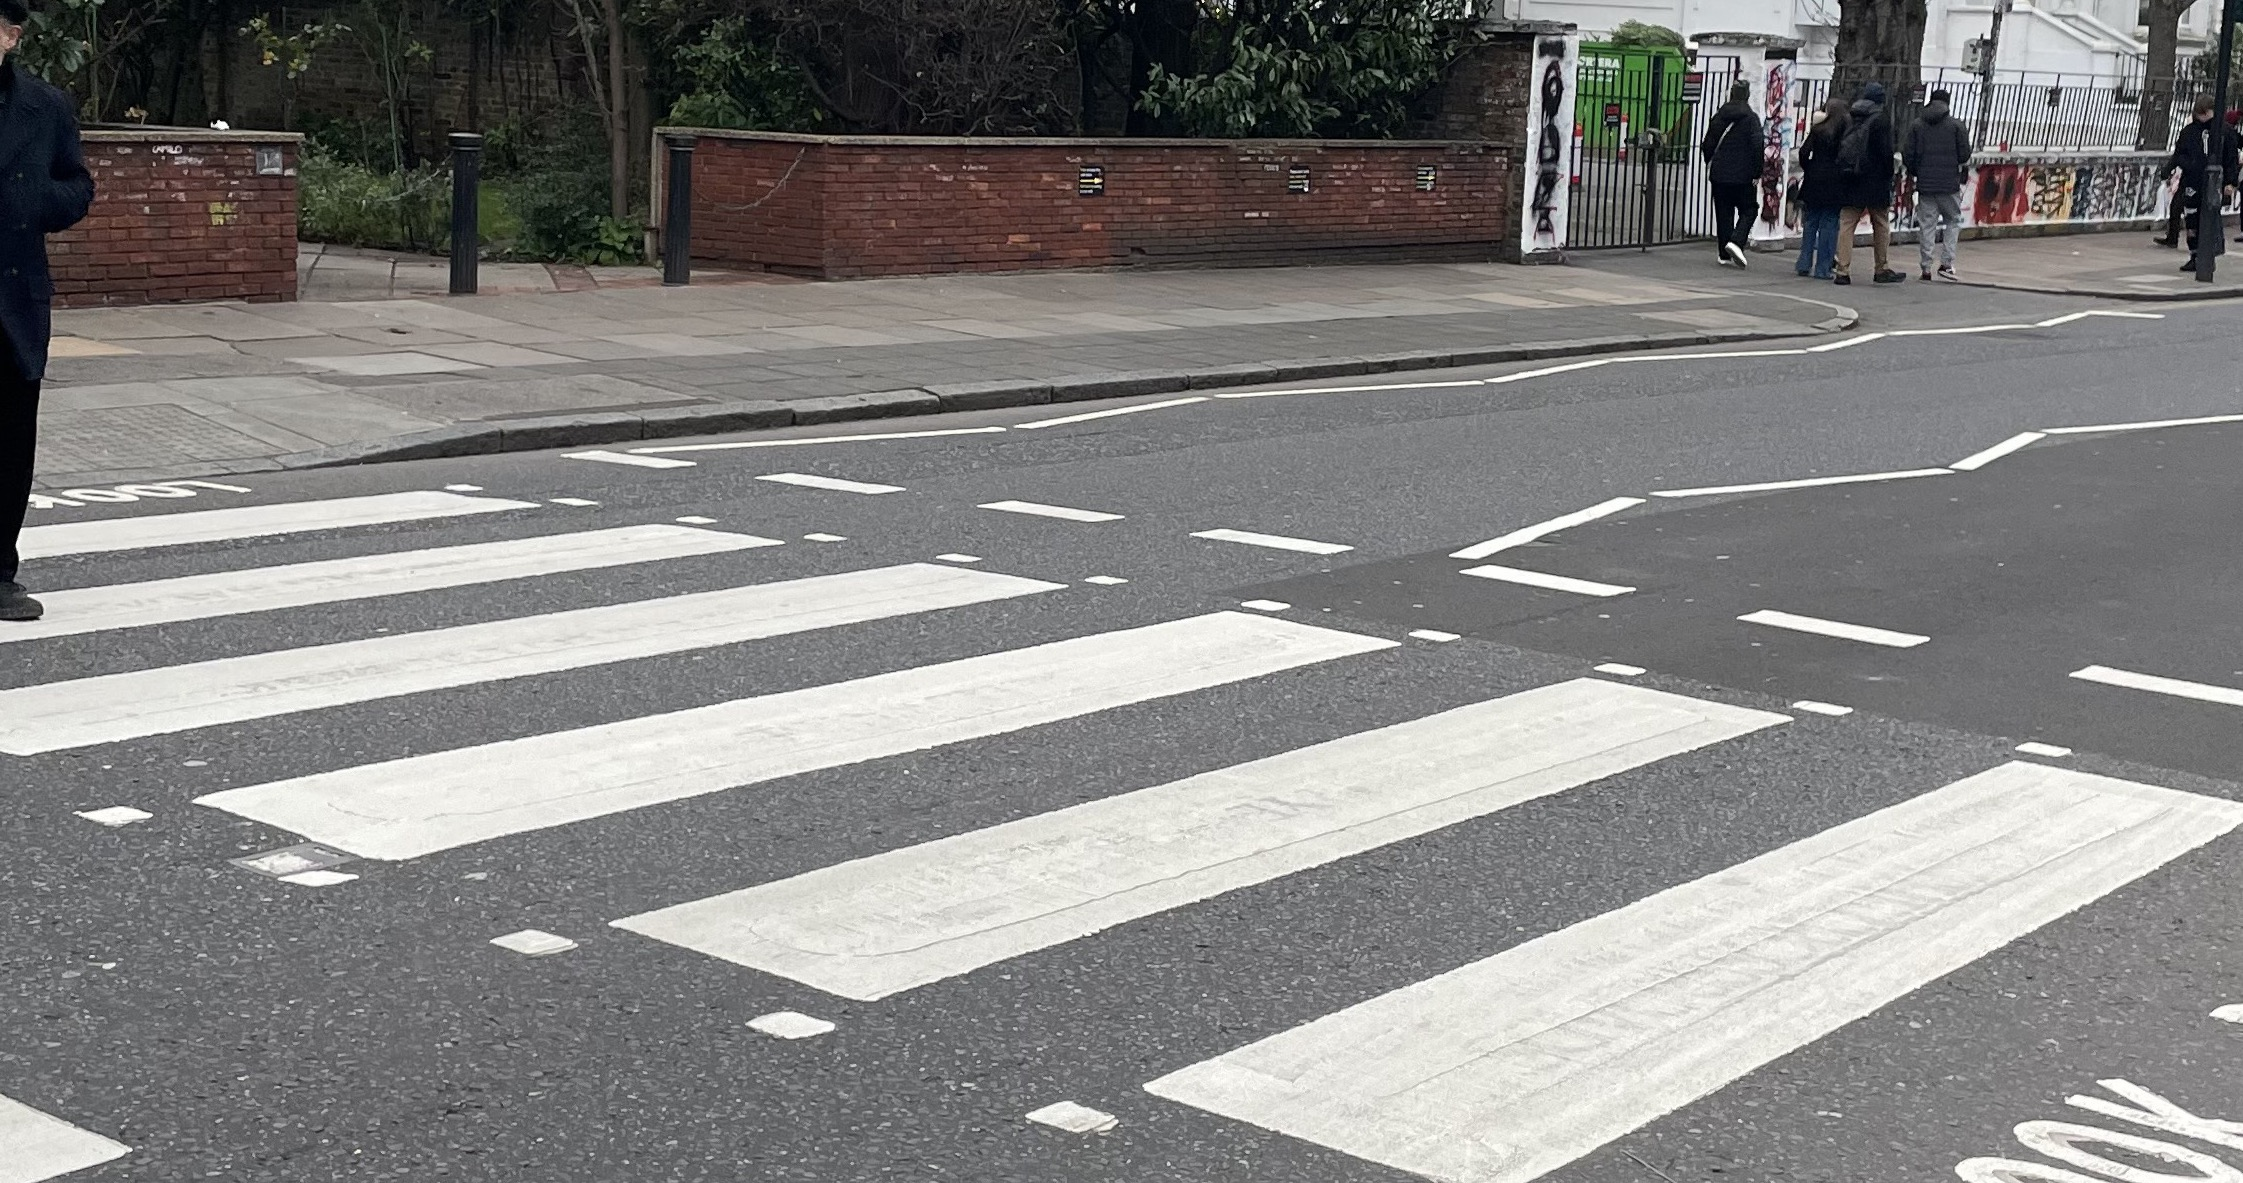
\includegraphics[width=0.5\linewidth]{
		\FIGURESPATH/AbbeyRoad.jpeg
		}
	\caption{
		Abbey Road, London, UK.
	}
	\label{fig:AbbeyRoad}
\end{figure*}

\subsection{Simulation Results}
\color{blue}\lipsum[1-2]\color{black}

\begin{figure}[!t]
    \centering
		\subfloat[
			Norm of weights $\hat\theta_i$.
		]{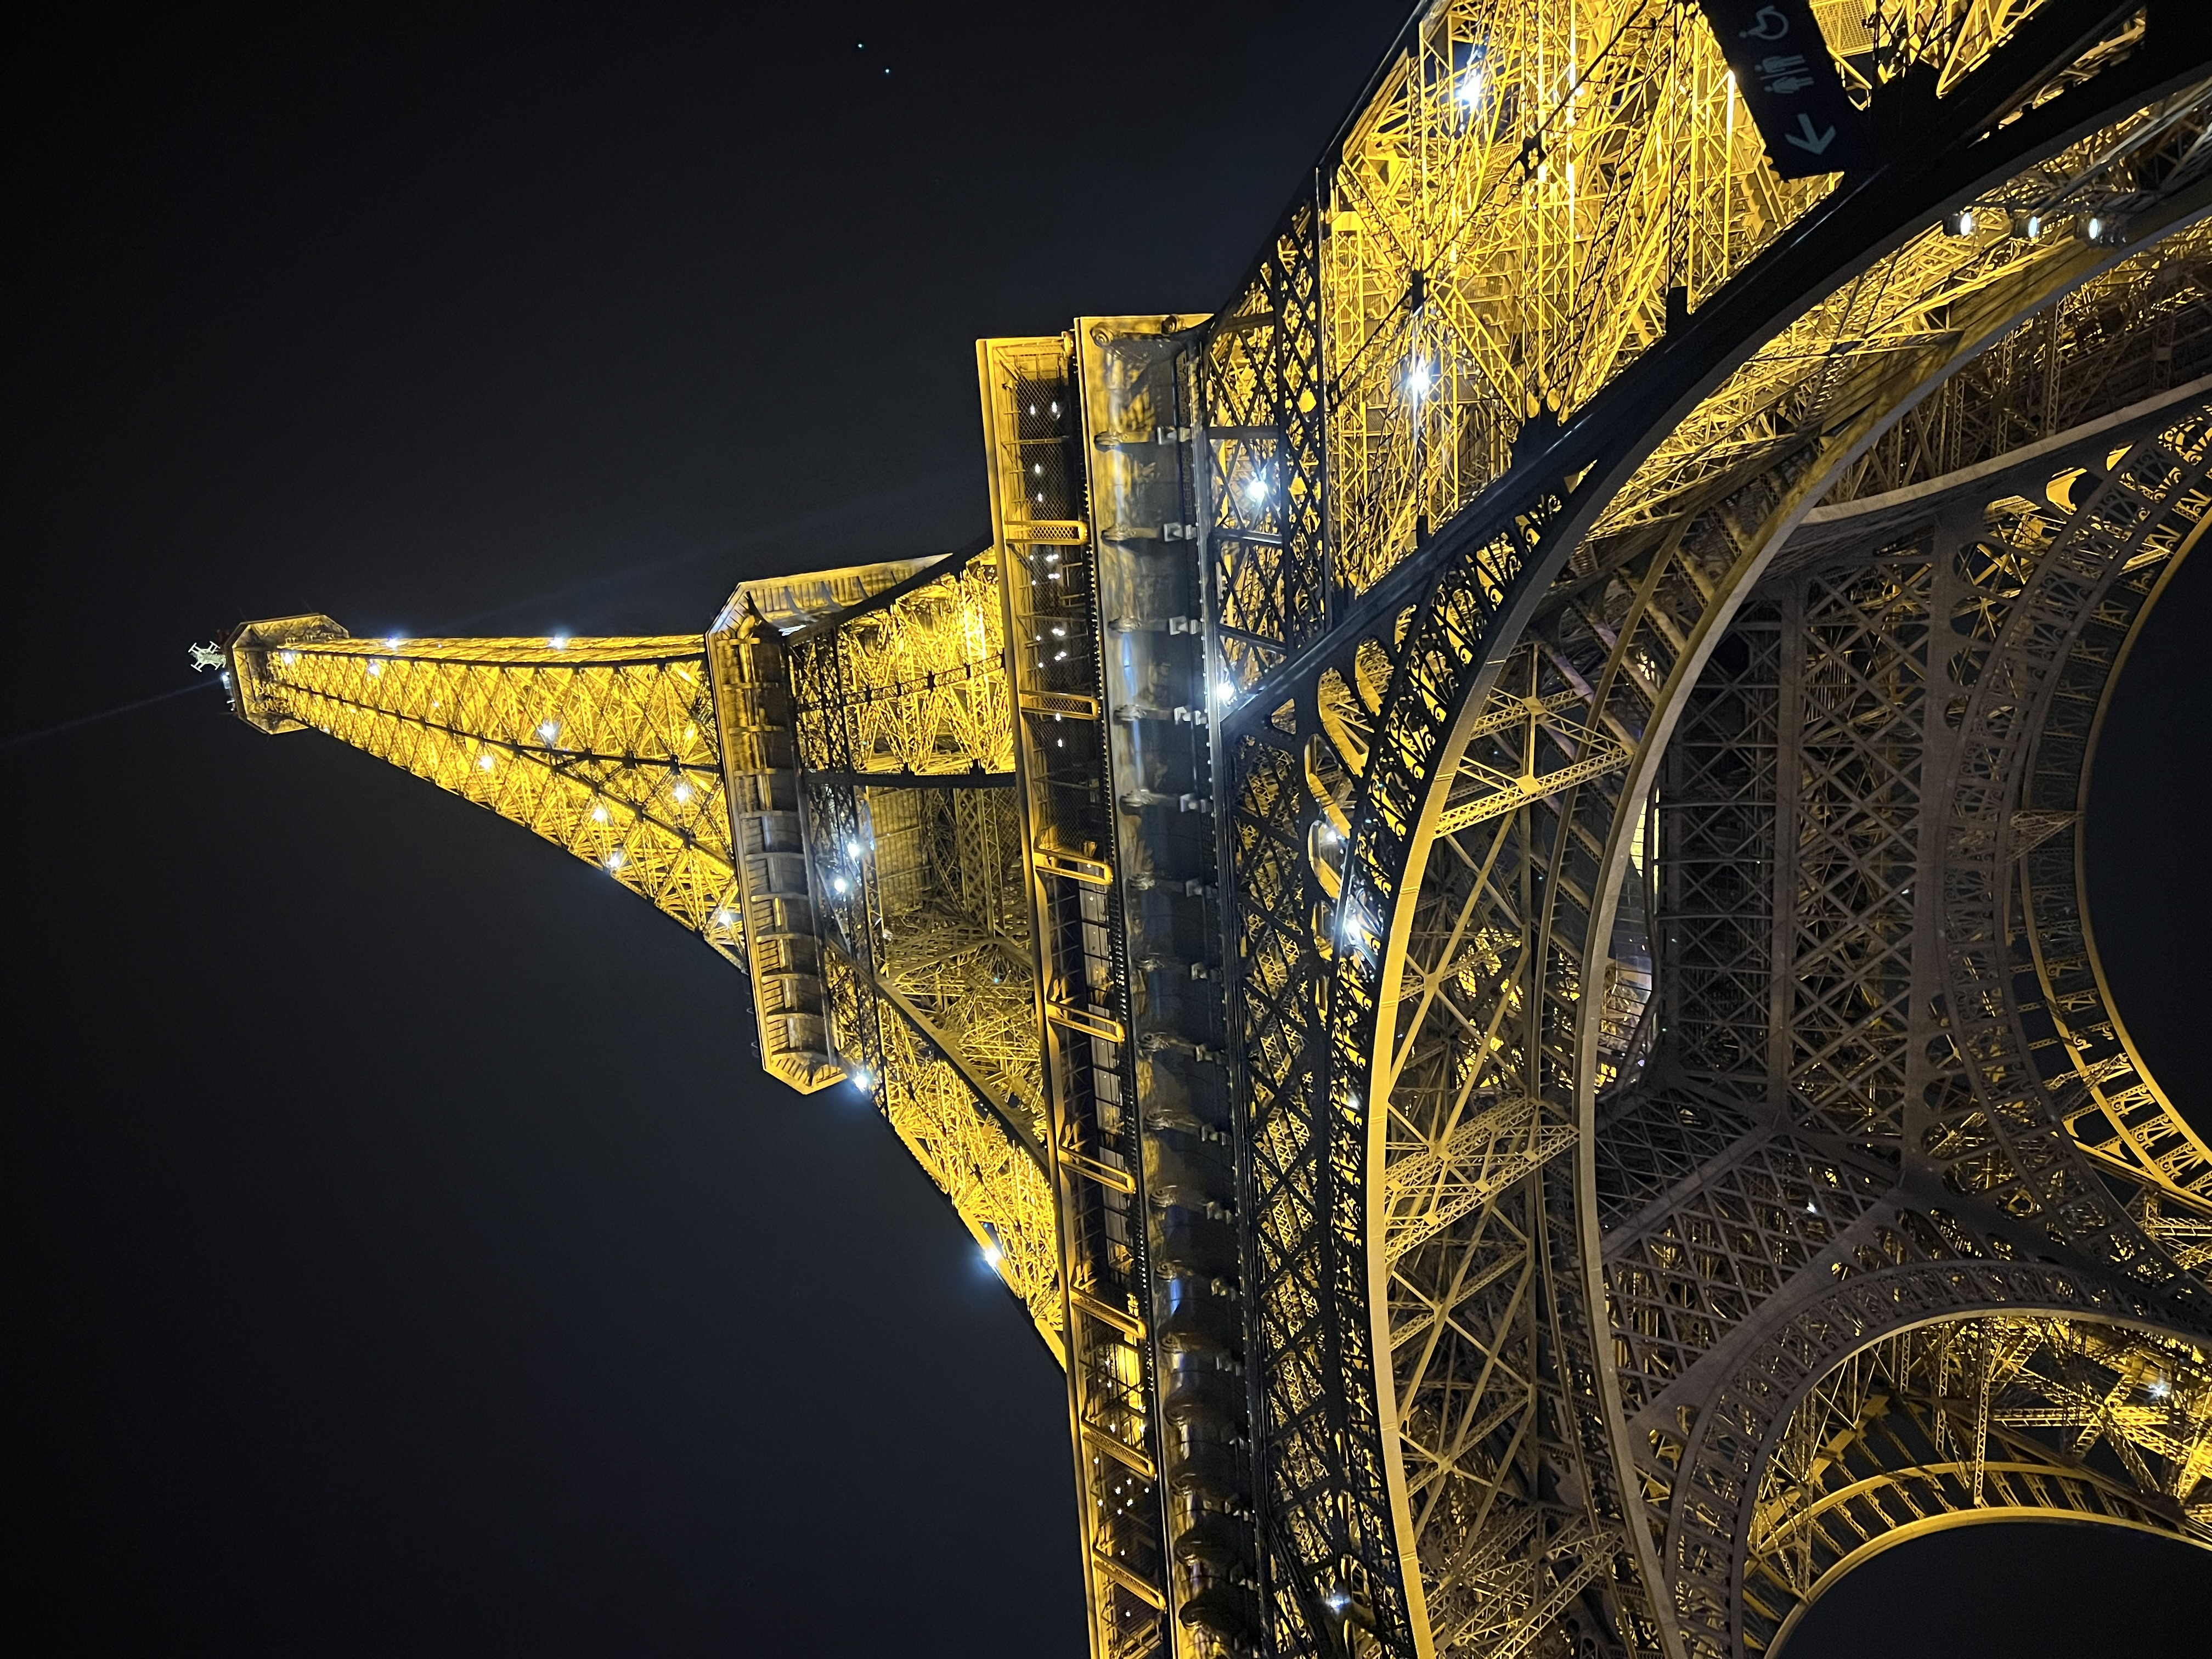
\includegraphics[width=0.99\linewidth]{
			\FIGURESPATH/Effel.jpeg
			}%
        \label{fig:weights_norm}}
	\vspace{1mm}
		\subfloat[
			Lagrange multipliers $\lambda_j$ in logarithmic scale.
		]{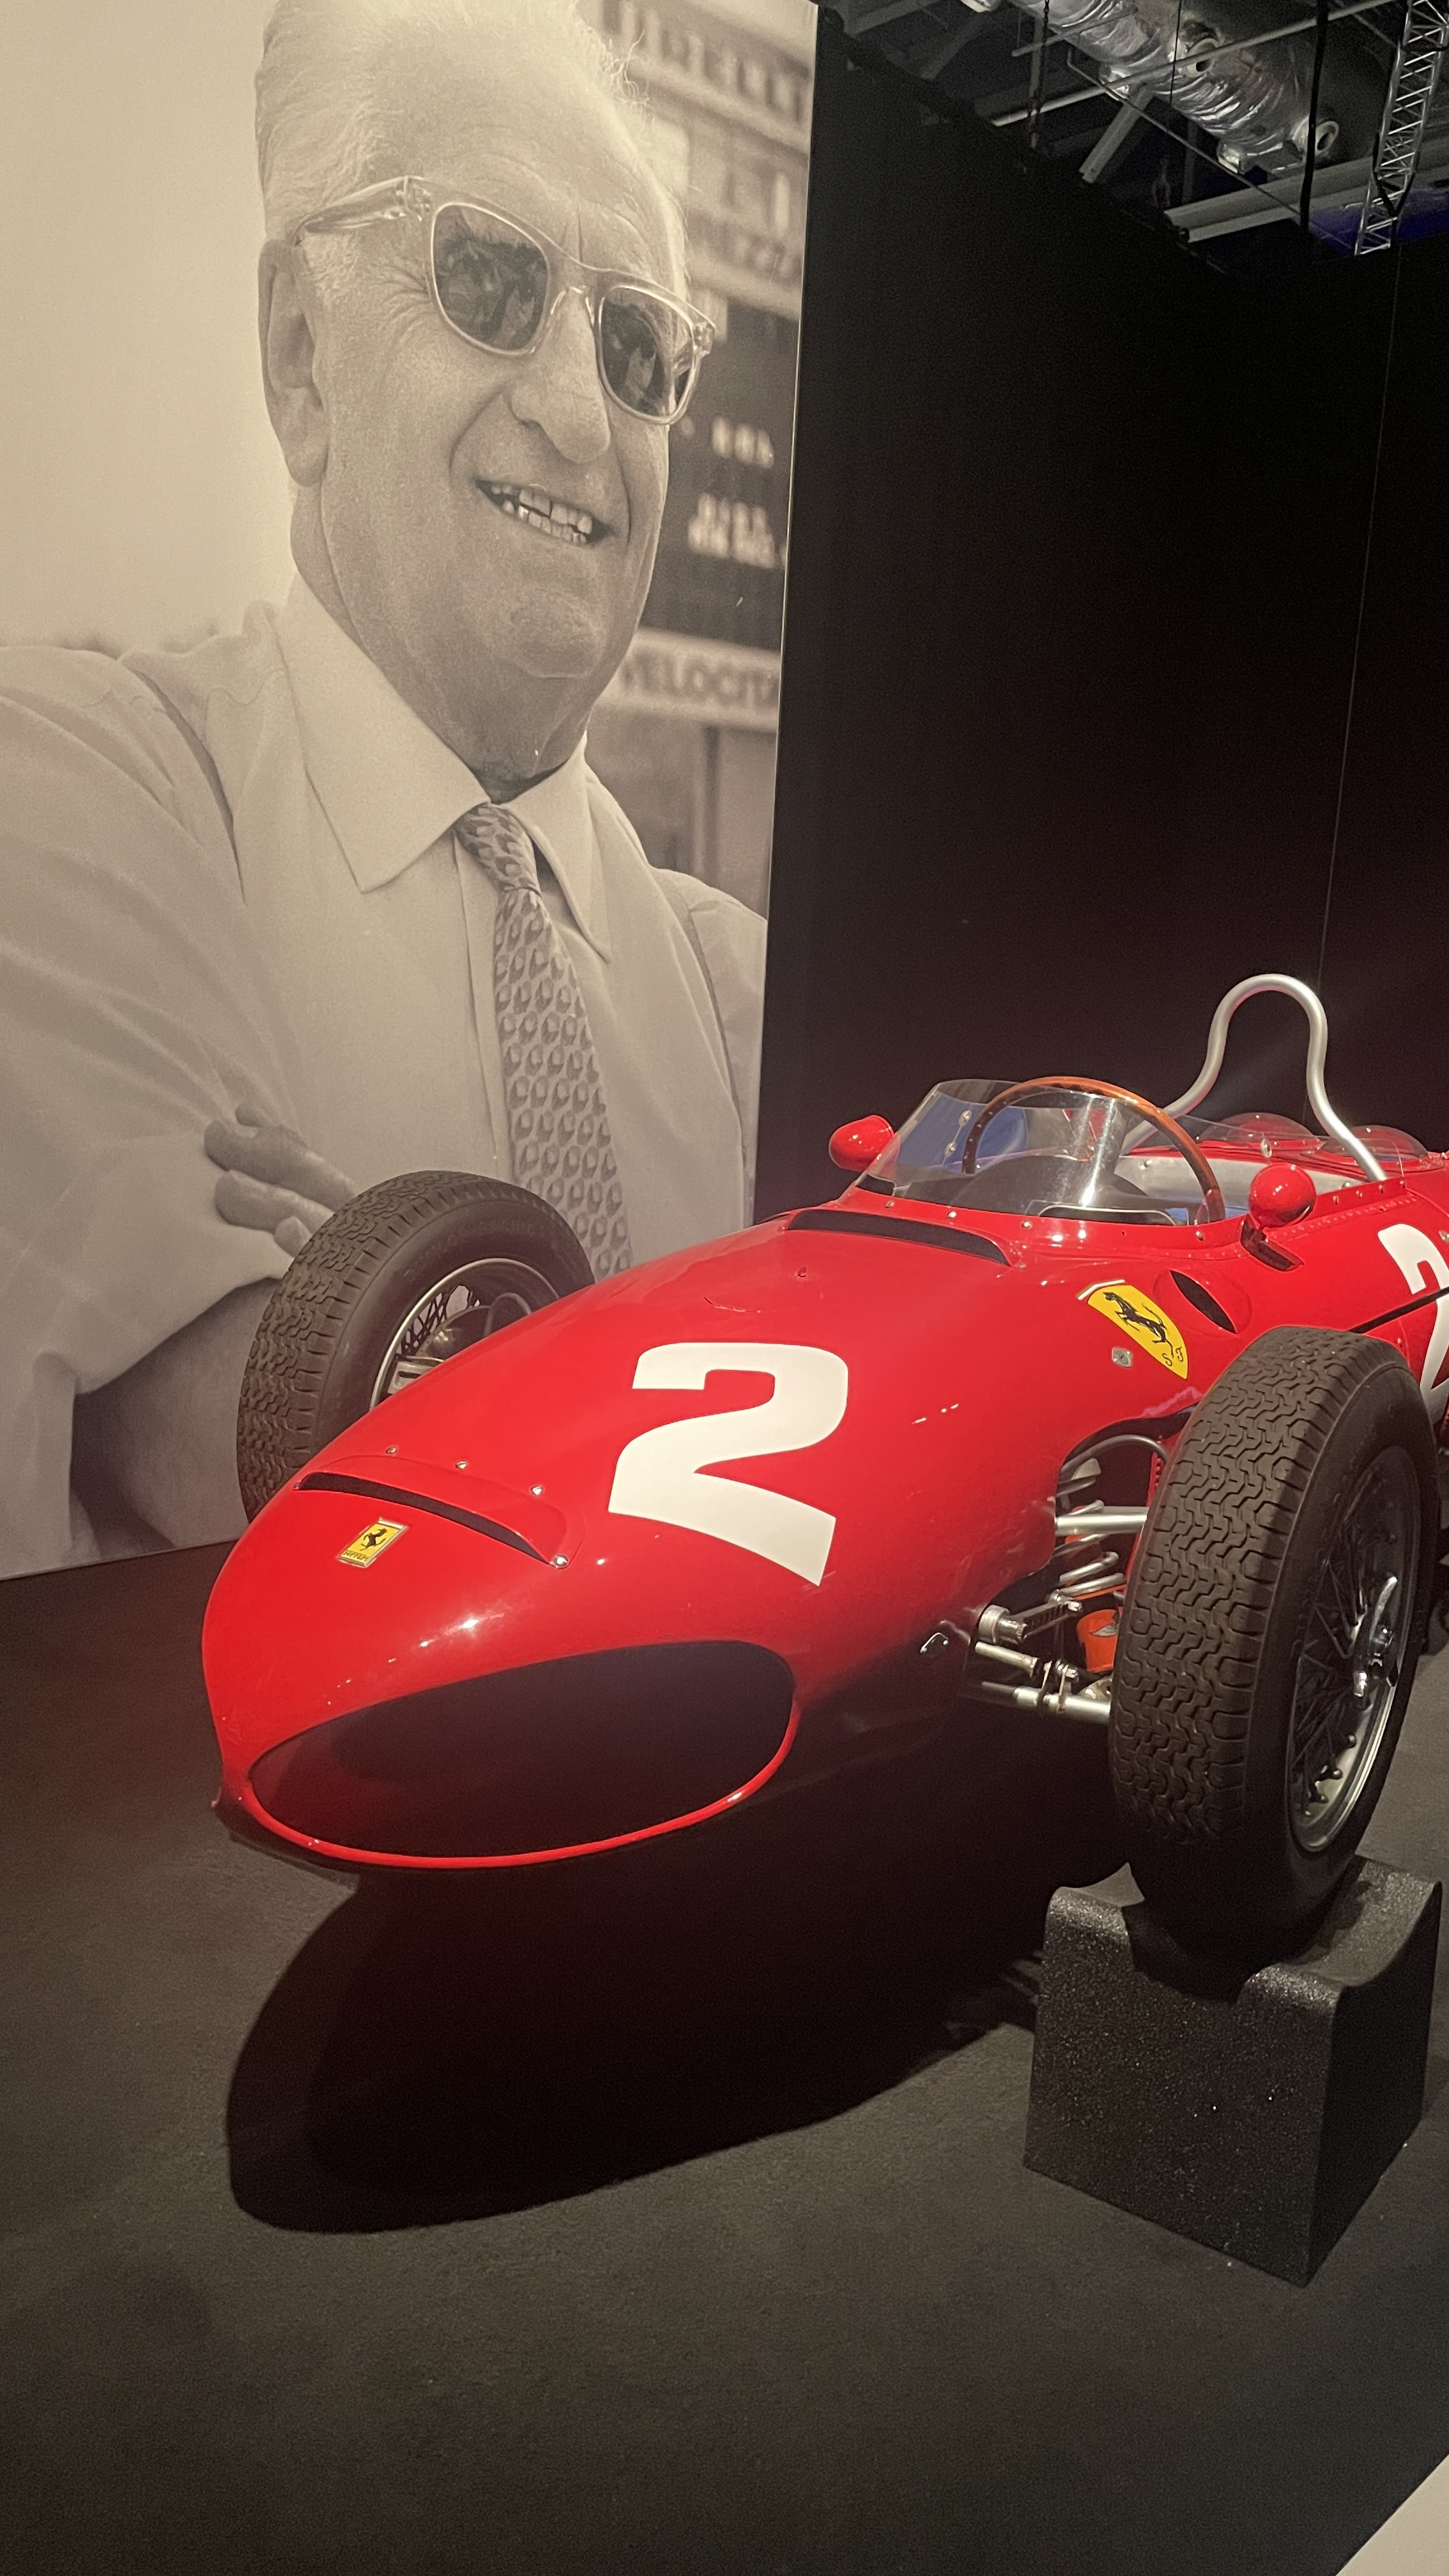
\includegraphics[width=0.99\linewidth]{
			\FIGURESPATH/Ferrari.jpg
			}%
        \label{fig:multipliers}}
    \caption{
		Hello
	}
	\label{fig:ctrl_result2}
\end{figure}

% ============================================
%            SECTION: Conclusion
% ============================================
\section{Conclusion}

\color{blue}\lipsum[1]\color{black}

% ============================================
%         BIBLIOGRAPHY
% ============================================
\bibliographystyle{ieeetr}
\bibliography{\template/refs}

\end{document}

